The research paper is connected with an area of study, called Mining Software Repositories (MSR)\cite{MSR2016}, that is growing together with the massive amount of available software repositories. Its purpose is to investigate and create relationships between the repository data items in order to find unique and useful information about a particular software system and, also, optimize the work that needs to be done during the analysis. Researchers and software developers use their own experience and knowledge for repository investigation and they tend to concentrate on a particular part of the code, e.g. testers usually are focusing on features errors and bugs. However, this might lead to faulty and ineffective results. MSR is an approach for overcoming this problem, it is analysing into great detail repositories and it is building complex models between data items\cite{hassan2008road}. IPython Observatory project is covering ideas and aspects that MSR is looking to achieve, with the difference that only a specific group of repositories are analysed - projects connected with IPython Notebook.

\subsection{GitHub limitations and data extraction}
\label{subsec:limitations}
The first part of the project is consisting of the creation of methods and techniques for the extraction of data from GitHub\cite{gitHubWiki} and the its limitations. Mining Software Repository field is concerned with the automation of gathering data from hosts such as GitHub. Two major problems that MSR is encountering are\cite{hassan2008road}:

\vspace{1em}
\begin{description}
    \item[Limited Access to Repositories]  Not all of the repositories are public, which means that they are available for everyone. Companies that are using GitHub as a version control service for their code are not interested of sharing details about their software systems, which makes research projects less effective since they can not access richer and more complex project than those that have less contributors and features\cite{hassan2008road}. 
    
    \item[Complexity of Data Extraction] A lot of time, effort and software knowledge is required to extract data from repositories. The new GitHub API (Application programming interface)\cite{GitAPI} is allowing access to a huge amount of repositories data. However, it has limitations for copying data and not all repository features are present. 
\end{description}
\vspace{1em}

IPython Observatory project faced the same limitations together with the collection of repositories that contain IPython Notebook scripts. Its prototype is extracting repositories that are containing the word \textit{IPython} with the help of the GitHub Search API\cite{GitAPISearch}, which sends and receives data as JSON\cite{json}. However, not all of search results are containing IPython scripts - that is an aspect that is considered in the research prototype. All of the analysis, explained in the next subsections, are done on repositories that have at least one IPython script. Also, the number and the content of repositories containing the word IPython are constantly changing - on November 2015 the number is 3933 and on March 2016 - 4492, which states that the usage of GitHub and IPython Notebook has increased in six months. The project's prototype is extracting data from the GitHub API and it is not tracking changes in time, which might be implemented as a future functionality.

Furthermore, the GitHub API is showing projects that are only publicly accessible. Analysis over repositories that have a huge number of commits and contributors are more likely to represent high quality of work and accuracy of results. The project encounters limitations with the extraction of data - Search GitHub API "provides up to 1,000 results for each search"\cite{GitAPISearch}, "for unauthenticated requests, the rate limit allows you to make up to 10 requests per minute"\cite{GitAPISearch} and the rate limit of the GitHub API is "60 requests per hour"\cite{GitAPI}. The prototype is downloading 866 repositories that contain the word "IPython" by an algorithm that is waiting a curtain amount of time on the ninth and fifty-ninth cloned repository. A future work for the project might overcome the GitHub API limitations and being able to analyse over all existing search results. 

The technique, used in the research prototype for extraction of data, is extracting the GitHub API JSON representation and it stores it into a file. Eaxh GitHub repository has url, which was used for cloning the projects. Python was used as a programming language for the code. The Python package GitPython\cite{GitPython} provides object model access to git repositories and it was used for cloning and analysing them. The limitations with the requests is handled by waiting 30 seconds on each ninth downloaded repository and waiting 30 minutes on every fifty-ninth downloaded repository. Since the GitHub API shows information only for one page of search results, the prototype is traversing through 10 pages(each page can contain 30 or 100 results, and the code set the parameter for that to 100) by changing a parameter in the search url. 

Finally, another issue that might be encountered during the extraction of information is storage. The amount of data of the all the cloned repositories is 19GB. University of Glasgow has provided a server for the research project, that takes up to 90GB of data. 

To sum up, this stage of the project overcame the issues and limitations encountered with access, collection, amount and storage of specific group of repositories. Two approaches for future work are suggested - tracking changes and quality of data in time and extraction of all search results.

\subsection{Mining Repository's information}
\label{subsec:mining}

A lot of researchers are analysing the usage of programming tools on GitHub and what effect does the version control hosting site has on the improvement of software systems. The Kalliamvakou's paper \cite{kalliamvakoupromises} is investigating possible threats to the validity of researches involving software projects hosted on GitHub. They can be viewed as fundamental steps for analysing all of the repositories connected with IPython notebooks. Figure \ref{fig:perils} is showing the results of the paper. In the paper are described thirteen perils that pose potential threats to validity for studies involving software projects hosted in GitHub. Instead of accepting these repository's perils as aspects that need to be avoid, IPython Observatory is investigating them and reporting the results for the usage of IPython in GitHub. This section describes the steps taken for the analysis made on repositories' features.

\vspace{5mm}
\begin{mdframed}
\vspace{1px}
\textbf{Aspect \RNum{1}:}  A repository is not necessarily a project
\vspace{1px}
\end{mdframed}
\vspace{2mm}

As described in the Kalliamvako's paper\cite{kalliamvakoupromises}, GitHub is using the pull request development model for collaboration in a software development project. It is accepted that contributors are not making any changes into the main repository of the project and they are cloning the repository and making changes without interfering with others work. All of the new and changed files of repository are stored in a local branch, which later is inspected and pulled into the master branch by a member of the project's core team. After a code review, the contributors need to update their local branches with the new commits. This model represents repositories as base and fork repositories - respectively, the main repositories and those that are independently recording activities. Only the commits in the base repositories are tracked, which means that non-merged ones will be ignored.

The technique used in IPython Observatory for identifying if a repository is a project, is extracting all merges made into the repository. GitPython was used for the process and each merge in the package has a name and a stage, which represents conflicts during the merging. If a stage is zero then there were no conflicts, else - there were conflicts in the merge. Then the prototype is traversing through each merges' stage and calculating the percentage of merges without any conflicts against the number of all merges. However, when the code was executed on the extracted 866 repositories and it returned a value of 1.0, which means that all of the merges in the repositories have no conflicts. The algorithm could be improved and investigated even further as a future task. 

Another technique has been implemented that analyses each of the files in a repository and extracting their names. The extension of the file gives information about the type of the file and the language used in it. In order to identify each possible format, a data set has been created that contains various formats met in GitHub repositories - the python package \textit{linguist}\cite{linguist} contains most of the languages. Another computation in the process is calculating the percentage of repositories that contain only text/plain files and IPython scripts - 4,3786\%. This shows that only a small amount of projects has storage purpose and it states the assumptions that there are not software development projects. This idea can be extended further - e.g. the most used language together with IPython.

\vspace{5mm}
\begin{mdframed}
\vspace{1px}
\textbf{Aspect \RNum{2}:}  Most projects have low activity
\vspace{1px}
\end{mdframed}
\vspace{2mm}

One of the most crucial features of GitHub repositories are the commits - 20 times more than pull request and issues\cite{kalliamvakoupromises}. Kalliamvako's paper\cite{kalliamvakoupromises} suggests that GitHub repository's activity can be measured with the number of commits and the time of commits, which tracks the lifespan of a project. This will indicate the work done for the project and its usage on GitHub.

The prototype of the research is counting the number of commits of all extracted repositories. GitPython package is allowing the extraction of commits by the creation of a Repository object for a specific project - it requires the path of the repository storage location. 

Several analysis were performed to investigate the activity of projects on GitHub. The first is calculating the average value for a number of commits for a repository. The results show that it is 102.93, which indicates that on average a repository has high number of commits and shows large activity. The second calculation is showing the standard deviation\cite{stdWiki} of the various number of commits - 831.5, which is high and it presents that the data points are spread out over a wide range of values. The prototype generates a histogram of the probability of all the values for number of commits, which can be seen on Figure \ref{fig:histogram}. The values are spreading until value 18,319, but it is showing only until 1000(a histogram spreading until 18,319 is also generated). The figure shows that the probability for the values between 0 and 400 to be number of commits, is the highest from all of the data points - the most common number of commits for IPython repository will be between 0 and 400. As final and third analysis, the prototype finds for every repository the date of the last commit and it looks for repositories that has finished productivity in year 2015 or 2016. This is one more indicator for project's activity. The investigation shows that around 58\% of all the repositories have closed or are still continuing. 

\begin{figure}
\centering
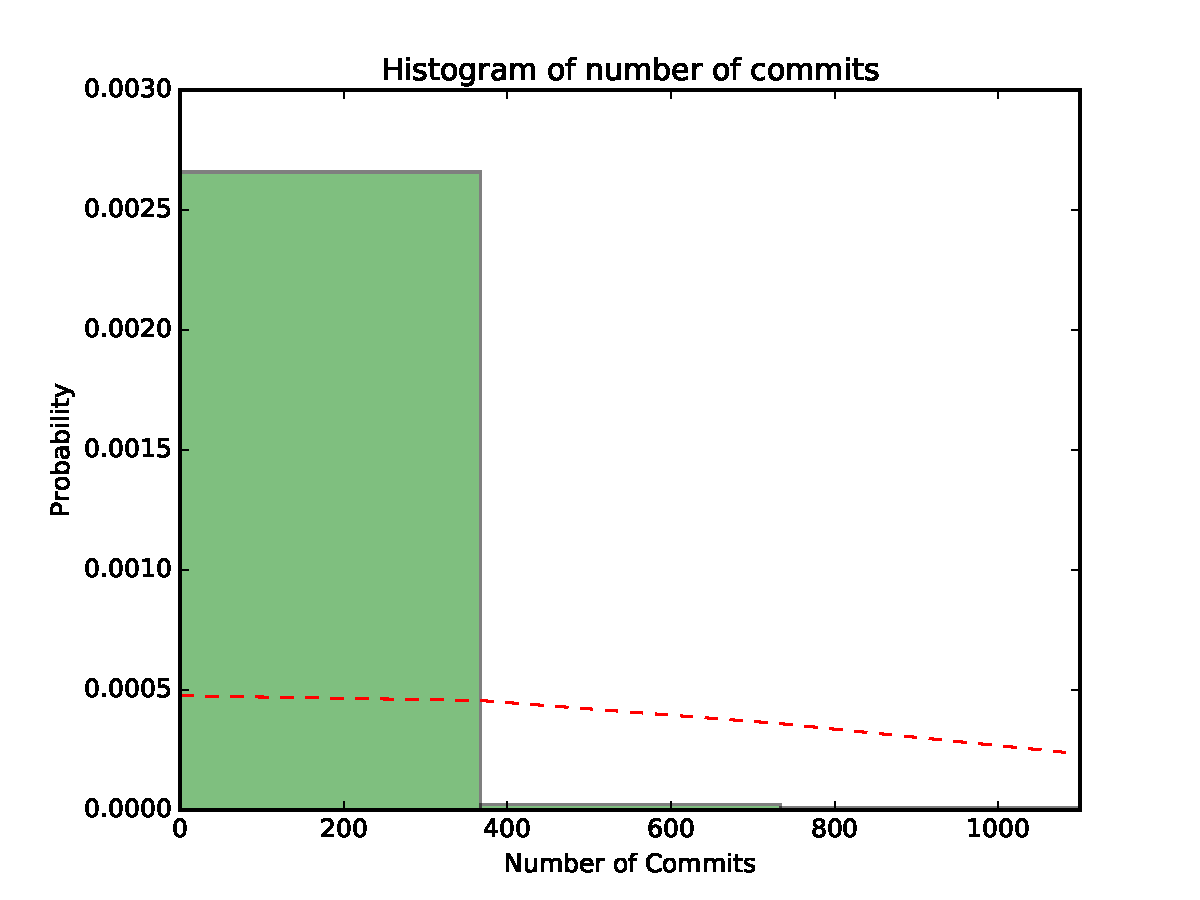
\includegraphics[width=0.4\textwidth]{images/commits_histogram_zoomed.pdf}
\caption{Activity of projects}
\label{fig:histogram}
\end{figure}

\vspace{5mm}
\begin{mdframed}
\vspace{1px}
\textbf{Aspect \RNum{3}:}  Most projects are inactive
\vspace{1px}
\end{mdframed}
\vspace{2mm}

This aspect is closely connected with the previous one - Aspect \RNum{2}. It is considered that if a project has a small number of commits, it would have limited functionality and it is inactive. In this part of the analysis the prototype is calculating the number of repositories that has not more than 10 commits - it is a small number for specifying repository's activity and there is no specific reason for its selection. The outcome of the computation is around 48\% of all repositories are assumed to be inactive. However, this process is based on assumptions and it can be extended further. An idea, which can be implemented in the future, is identifying the most appropriate number or model as an indicator of low activity, depending on the variety of commits in a repository. 

\vspace{5mm}
\begin{mdframed}
\vspace{1px}
\textbf{Aspect \RNum{4}:}  Many projects are not software development
\vspace{1px}
\end{mdframed}
\vspace{2mm}

Kalliamvako's survey\cite{kalliamvakoupromises} reports that GitHub repositories are not only used for software developement projects - 14\% respondents (out of 240) are using GitHub for experimentation's and academic/class projects and 10\% are using it for storage. IPython Observatory's idea originates from the idea that GitHub repositories are used for various purposes - e.g. storing IPython notebooks for teaching, learning and organizational purposes. 

IPython Observatory is is analysing two aspects of a repository in order to identify the usage of IPython - languages used in a repository - types of files and whether a repository has a README file or similar describtion file. One more aspect to be considered for future implementations might be the content of a README file - implementing an algorithm for identifying the aim of the project explained in the README file. 

The research has developed the idea of finding and analysing all of the licenses and README files with the Python package \textit{textstat}\cite{textstat}, which helps with the calculation of statistics from text by deciding readability, complexity and grade level of a particular corpus. Also, the technique of finding the files is based on a data set that contains different formats of the README and license files - e.g. not all of them are text files. The data set is created from manually exploring the most common presentations of the files.

Furthermore, if a repository is used for only storage purposes, it might only has few number of commits and a small lifespan. This contradicts with the statement that we made above - if a project has small amount of commits then it is more likely to be inactive. A future implementation for analysis could be the creation of a model between these two aspects or any other two aspects - Aspect \RNum{3} and Aspect \RNum{4} paragraphs.


\vspace{5mm}
\begin{mdframed}
\vspace{1px}
\textbf{Aspect \RNum{5}:}  Most projects are personal
\vspace{1px}
\end{mdframed}
\vspace{2mm}

A GitHub repository might have one or several contributors - it could be used not only for collaboration, but also for personal use, which connects with the idea mentioned in Aspect \RNum{4}, that some projects might be used only for storage. Kalliamvako's survey\cite{kalliamvakoupromises} reports that 38\% out of 240 respondents use GitHub mainly for their own projects and they don't have the intention of collaborating with others. The result are an motivating factor for analysis over the collaboration and social interaction in IPython Notebook's projects. 

IPython Observatoiry evaluates if a project is personal by counting the number of different committers in all the collected repositories. GitPython implementation has a Commit object, which contains different information for commits, such as author and date. The prototype is extracting all commits and extracting different authors from commits for each repository. Afterwards, its calculating the repositories with only one committer - around 42\% of all repositories, and those with one or two committers - around 63\%. The results show that more than half of the projects are personal. 

Also, the Kalliamvako's survey\cite{kalliamvakoupromises} results show that most of the projects on GitHub are used by only one person, most likely for experimental or storage purposes. An idea for analysis over the relation between the usage of IPython projects for personal use and all repositories on GitHub for personal used, might be implemented as a future improvement.


\vspace{5mm}
\begin{mdframed}
\vspace{1px}
\textbf{Aspect \RNum{6}:}  Many active projects do not use GitHub exclusively
\vspace{1px}
\end{mdframed}
\vspace{2mm}

GitHub allows contributes on a project not only for registered users. Analysis over the type of contributors of a project indicates areas of usage for a specific project. IPython Observatory has chosen GitHub as the most popular and changing source of information, but there might be others. There are two aspects that helps with the investigation over this aspect and they could be considered as future work - survey of users using both IPython and a host service, and analysis over the names of the contributors in a specific IPython project - if a non GitHub user made a commit, then GitHub records an email address as their work\cite{kalliamvakoupromises}. Kalliamvako's survey\cite{kalliamvakoupromises} concludes that there is a huge number of projects, which activities are not conducted within GitHub.

\vspace{5mm}
\begin{mdframed}
\vspace{1px}
\textbf{Aspect \RNum{7}:}  Many active projects do not use GitHub exclusively
\vspace{1px}
\end{mdframed}
\vspace{2mm}

Kalliamvako's paper\cite{kalliamvakoupromises} reports that personal projects, which are 67\% from all of the projects, and they are not using pull requests. This aspect is connected with Aspect \RNum{7} and it could use the same approach for analysis and include one more functionality - number of pull requests, since personal projects should have zero pull requests.

\vspace{5mm}
\begin{mdframed}
\vspace{1px}
\textbf{Aspect \RNum{8}:}  Merges only track successful code
\vspace{1px}
\end{mdframed}
\vspace{2mm}

The peer review model on GitHub has a disadvantage for the project's commits - they might not be readily-observable. This means that usually, all the commits are reviewed and merged within the main repository as one. The GitHub API\cite{gitHubAPI} is recording only the final stage and not all of the original commits. As a consequence, researchers can only observe the latest commit, which is the outcome of the code review process\cite{kalliamvakoupromises}.

IPython Observatory is analysing through this aspect of a repository by extracting all merges that are accessible for a repository. It is closely connected with Aspect \RNum{2} and Aspect \RNum{9}. The process, extracting the repositories' merges and their stages(Aspect \RNum{2}), is supporting the investigation for tracking successful code.  

\vspace{5mm}
\begin{mdframed}
\vspace{1px}
\textbf{Aspect \RNum{9}:}  Many merged pull requests appear as non-merged.
\vspace{1px}
\end{mdframed}
\vspace{2mm}

Merged pull requests might be merged outside GitHub, as explained in Aspect \RNum{8}. Kalliamvako's paper\cite{kalliamvakoupromises} has developed a heuristics based on conventions advocated by GitHub. Creation of a prototype that implements these heuristics might be considered as a future work and it will contribute to the field of Mining Software Repositories(MSR) \cite{MSR2016}.

\vspace{8mm}

Aspects \RNum{10}, \RNum{11} are closely connected with Aspect \RNum{6}. IPython Observatory has conducted analysis over number of contributors for a specific project. They can be extended into a lot more complex models and into software tools that implement the models. 

Aspects \RNum{12}, \RNum{13} are specific for the Kalliamvako's paper\cite{kalliamvakoupromises}. They are suggested analysis over the whole information that can extracted from GitHub. With respect to IPython projects, Aspects \RNum{12}, \RNum{13} might be understood as points that are covered in subsection \ref{subsec:limitations}.



Amongst high-level open source programming languages, Python is today the leading tool for general-purpose source scientific computing, finding wide adoption across research disciplines, education and industry \cite{perez2013open}.

Python is effective programming language for converting scientific code from another language \cite{perez2013open}. It was created not only for application of simple calculations and operations. Python can become a high-level language, which can be used in software engineering or scientific environments. Additional extensions for Python are created everyday and they are available and understandable for everyone \cite{sanner1999python}.

\subsubsection{Python Facilities for Scientific Programming}

A lot of scientific researches use Python for computing complex functions, which results in more accurate calculations and predictions than measuring them manually. Python has not been widely used in statistical measurements, but nowadays various scientists find its usage effective and powerful. With the creation of libraries, such as Matplotlib \cite{matplotlib}, NumPy \cite{numpy} and SciPy \cite{scipyOff}, Python has became one of the most preferred software tools for research, testing and engineering \cite{perez2007ipython}. There many more examples for the usage of Python package libraries, such as SkLearn - package containing implementation of various machine learning algorithms, and OpenCV - image processing and analysis. \cite{sklearn}\cite{openCV}

Data visualizations are great practice for conducting accurate analysis - they show relations between data items and objects. Python has made enormous contribution to their development and broad usage. For example, IPython Notebook is an interactive tool for combining and styling text and code concurrently. Also, parallel processing with processes and threads, Interprocess communication (MPI), GPU computing, have found great support from Python programming.

This section is explaining how researchers have tried to assess the usage of Python in scientific computing. There are a variety of approaches and methods for determining the easiness of features in Python - the best of them is the practical use of Python in different cases. SciPy conferences subsection is describing the experiences of analysts with Python. 

\vspace{2mm}
\paragraph{Syntax and structure of Python code} 
\label{syntax}
\vspace{3mm}

In this subsection we are mainly going through one article, Oliphant's \cite{oliphant2007python}, from other research documentation. 

High-level languages can enormously increase productivity and that is why they have been used for scientific computing for many years. Countless analysts and researchers have found these language to be of great use for them, since they are facing tasks of implementing nontrivial computational software prototypes in order to prove a concept for their area of exploration. Python is one of these languages and it allows engineers to be more careless with syntax, error handling and compilation time. However, comparing it with other languages, Python presents more effective environment for scientific applications.

Travis Oliphant's article continues by listing the basic features of Python: liberal open source license - allows selling, using, or
distributing of Python-based applications, Python running on many platforms - no concerns about writing an application with limited portability, the language's clean syntax - object-oriented coding, depending on the situation, a powerful interactive interpreter - allows code development and experimentation, and others.\cite{oliphant2007python}

All of the above features are useful for implementing scientific computations with Python. Travis Oliphant goes into more detail about the clean syntax, useful built-in objects, functions and classes, standard library, ease of extension, and the importance of libraries, such as NumPy and SciPy. With examples, he is able to show that only with a few lines of code, a complex functionality can be implemented, and errors, failures and bugs can be caught. 

The Travis Oliphant's paper\cite{oliphant2007python} provides a "small taste" of Python's usefulness and he is going through the language itself. The author is supporting the argument that Python is beneficial by starting with the syntax, which makes the code easy to understand and maintain, continuing with more examples for the built-in scalar types and the prepackaging libraries, and ending with SciPy package's calculation and computational ability. The structuring and syntax of the programming scripts is an important part since the concentration of a researcher will be mainly focused on the accuracy of the calculations and the discovery that was made, than in the validity of the code. With Python both features can be complete. 

The article argues that Python is clear to read, study and apply in various software applications. However, it is not going through a lot of detail for execution and compilation time \cite{HansPython}. Since Python is an interpreted language, it runs many times slower than compiled code. Then why we should consider using it in scientific complex functions? The next paper reviewed considers of the performance of Python.\ref{performance}

\vspace{2mm}
\paragraph{Performance of Python}
\label{performance}
\vspace{3mm}

Python must be compiled before it is run - it differs from C, C++ and other languages. Python programs are scripts - instead of having compilation process, Python is interpreted line-by-line. The positive side of it is the code flexibility for problem solving. However, if a complex functionality is implemented with Python rather than with some other compiled language, it will run slower. We are returning again to the question - why should we use such a time-consuming programming language in scientific computing? \cite{ScottPython}

 Hans Fangohr's paper \cite{HansPython} gives two answers to that criticism - implementation time versus execution time, and well-written Python code can be very fast.

The paper argues that not only the computational time has to be considered in the overall time for the whole process of scientific software prototype's implementation. Since the first scientific computing, the computer's processing has increased significantly. Also, it is of great importance how the code will be written, maintained and how number lines of code it will contain. If the code is short, there is a possibility for less errors and failure, and it gives faster approach for testing and maintenance. Another observation is that Python has a reliable interface to binary code - Cython.  So you can express the program in high level code and have the performance critical bits executed directly in binary.

The Cai's and Xing's article \cite{cai2005performance}, addresses the performance of scientific applications that use the Python programming language. It introduces several algorithms for increasing the efficiency of serial Python codes, after which it goes into detail for parallelization of serial scientific applications. The result is that if the code, for array-based operations, is written efficiently and it is able to achieve satisfactory parallel performance. As mentioned in \ref{syntax} Python is good for combination with other programming languages, such as C and C++, which means that great serial and parallel performance can be achieved by writing small, well defined, critical parts of a code in a lower level language. 

The Cai's and Xing's paper \cite{cai2005performance} compare Python with several languages, such as MatLab, Octave, Fortran, C and others, since each of these has its own advantages in term of performance and execution time. Python appear to be one of the most competitive alternatives for scientific computations. Compared with MatLab, Python also has the feature of numerical and visualization modules, which makes it so influential and dynamic. As an object-oriented language that allows handling of errors and failures, mixed-language support and cross-platform interface, it is possible to write highly readable code \ref{syntax}. Unlike MatLab, Python's creation of classes is more convenient, which is one of the reasons that researchers are using interpreted scripting language over a compiled one.

Python has been applied in various range of areas, not only in scientific researches. It can been use for web scraping, system administration, web development, distributed systems, computational steering, search engines and many others. \cite{cai2005performance} Scientific researches need a lot of background from different areas of exploration so that they can conclude the most accurate results. Powerful software tool that enables a broad range of tasks, as the ones mentioned in the previous paragraph, will be effective and efficient engine for achieving unique outcomes. 

Since, the core of Python is not sufficient for scientific computations with complex and demanding computations, with the creation of NumPy library, array data structures and long nested loops are processed faster and more smooth than before. It, also, includes multi-dimensional array structures with a lot of methods for accessing or changing them. NumPy's features appear to be as a "mirror" of MatLab's ones. 

The paper, also, investigates the capabilities of Python for parallel programming applications \cite{cai2005performance} With a lot of examples given, Python can be used in parallel computations, where the issues of data partitioning and structuring can be handled. It is "fast enough" for most computational tasks. Its readability and the re-usability of the code hide the fact that Python has reduced speed compared to other languages. 

Python is a compiled language and Xing Caia's paper \cite{cai2005performance} 
is proving that some programming languages, such as C++ might be more flexible and elegant than Python, but \textit{"...Python is much more convenient, and convenience seems to be a key issue when scientists choose an interpreted scripting language over a compiled language..."} \cite{cai2005performance} The research is evaluating the performance of parallel Python code in a real scientific application, which is compared to C code. The both serial and parallel performances are equal. In terms of efficiency and optimization Python is helpful for mathematical functions.

\vspace{2mm}
\paragraph{SciPy conferences} 
\label{SciPy}
\vspace{3mm}

In the previous section we analyze the usage of Python in scientific computing. But how does researchers and scientists see the Python code? What kind of experience they gain from it? This section is covering several SciPy conferences with real life examples, experiences and opinion of people that are using Python in the field of scientific programming.

For some people, it is not clear why Python has become the language of choice for so many people in scientific computing. Maybe if researchers like Travis Oliphant had decided to use some other language for scientific programming years ago, we'd all be using that language now. Python wasn't intended to be a scientific programming language. And as Jake VanderPlas points out in his keynote, Python still is not a scientific programming language, but the foundation for a scientific programming stack. Maybe Python's strength is that it's not a scientific language. It has drawn more computer scientists to contribute to the core language than it would have if it had been more of a domain-specific language.

John Cook reported his experience of migrating from Ruby and other scripting languages to Python. As a mathematician, he needed to start doing computational functions. He describes that period of transferring as \textit{"a rude awakening"}.\cite{johnSciPy} As soon as he started programming on Python, he found that the language provides \textit{"a hoard of code"} \cite{johnSciPy}, which includes a lot of libraries for various kind of data analysis. The comparison that he makes between languages, such as MatLab and R, and Python is the best description of the difference between them:

\textit{"I'd rather do mathematics in a general programming language than do general programming in a mathematical language."}

He is aware that the most acknowledged disadvantage of Python is its lack of speed, but for John Cook finds even harder rewriting code in other language. 

The conference, by Kelsey Jordahl \cite{efficientPython}, provides a tutorial on open source tools for using geospatial data in Python. It is a great example of Python being useful and incredibly effective for analyzing data in a specific area of study. The tutorial is going through the fundamental geological libraries of Python, such as reading vector data with Fiona - minimalist python package for reading (and writing) vector data in python, and geometry with Shapely - Python library for geometric operations using the GEOS library. 

Another helpful SciPy conference is by Mike McKerns \cite{efficientPython}. It is a tutorial that provides examples and essential performance tips for writing effective parallel Python - one more prove for the usefulness of Python. The tutorial could be found on GitHub \cite{parallel}. The conference is supporting the findings in the Cai's and Xing's paper \cite{cai2005performance}. SciPy conferences are not only great for teaching and practicing Python coding, but also they going through important research findings. \cite{sciPy} 


\subsubsection{Summary}
This literature review is investigating the usage of Python and it is showing how easy and efficient it is for your daily computational work. Python can be of great help even in small scripts with numerous data structures, classes, nested loops, documentation and others. Python has open source libraries, such as Numpy, SciPy, IPython for interactive work and MatPlotLib for plotting, which makes writing code quickly for machine learning and artificial intelligence. For a small amount of time, everyone can learn Python and apply powerful data structures and design patterns when needed.

